\documentclass[journal, a4paper]{IEEEtran}

% some very useful LaTeX packages include:

\usepackage{hyperref}

%\usepackage{cite}      % Written by Donald Arseneau
                        % V1.6 and later of IEEEtran pre-defines the format
                        % of the cite.sty package \cite{} output to follow
                        % that of IEEE. Loading the cite package will
                        % result in citation numbers being automatically
                        % sorted and properly "ranged". i.e.,
                        % [1], [9], [2], [7], [5], [6]
                        % (without using cite.sty)
                        % will become:
                        % [1], [2], [5]--[7], [9] (using cite.sty)
                        % cite.sty's \cite will automatically add leading
                        % space, if needed. Use cite.sty's noadjust option
                        % (cite.sty V3.8 and later) if you want to turn this
                        % off. cite.sty is already installed on most LaTeX
                        % systems. The latest version can be obtained at:
                        % http://www.ctan.org/tex-archive/macros/latex/contrib/supported/cite/

\usepackage{graphicx}   % Written by David Carlisle and Sebastian Rahtz
                        % Required if you want graphics, photos, etc.
                        % graphicx.sty is already installed on most LaTeX
                        % systems. The latest version and documentation can
                        % be obtained at:
                        % http://www.ctan.org/tex-archive/macros/latex/required/graphics/
                        % Another good source of documentation is "Using
                        % Imported Graphics in LaTeX2e" by Keith Reckdahl
                        % which can be found as esplatex.ps and epslatex.pdf
                        % at: http://www.ctan.org/tex-archive/info/

%\usepackage{psfrag}    % Written by Craig Barratt, Michael C. Grant,
                        % and David Carlisle
                        % This package allows you to substitute LaTeX
                        % commands for text in imported EPS graphic files.
                        % In this way, LaTeX symbols can be placed into
                        % graphics that have been generated by other
                        % applications. You must use latex->dvips->ps2pdf
                        % workflow (not direct pdf output from pdflatex) if
                        % you wish to use this capability because it works
                        % via some PostScript tricks. Alternatively, the
                        % graphics could be processed as separate files via
                        % psfrag and dvips, then converted to PDF for
                        % inclusion in the main file which uses pdflatex.
                        % Docs are in "The PSfrag System" by Michael C. Grant
                        % and David Carlisle. There is also some information
                        % about using psfrag in "Using Imported Graphics in
                        % LaTeX2e" by Keith Reckdahl which documents the
                        % graphicx package (see above). The psfrag package
                        % and documentation can be obtained at:
                        % http://www.ctan.org/tex-archive/macros/latex/contrib/supported/psfrag/

%\usepackage{subfigure} % Written by Steven Douglas Cochran
                        % This package makes it easy to put subfigures
                        % in your figures. i.e., "figure 1a and 1b"
                        % Docs are in "Using Imported Graphics in LaTeX2e"
                        % by Keith Reckdahl which also documents the graphicx
                        % package (see above). subfigure.sty is already
                        % installed on most LaTeX systems. The latest version
                        % and documentation can be obtained at:
                        % http://www.ctan.org/tex-archive/macros/latex/contrib/supported/subfigure/

\usepackage{url}        % Written by Donald Arseneau
                        % Provides better support for handling and breaking
                        % URLs. url.sty is already installed on most LaTeX
                        % systems. The latest version can be obtained at:
                        % http://www.ctan.org/tex-archive/macros/latex/contrib/other/misc/
                        % Read the url.sty source comments for usage information.

%\usepackage{stfloats}  % Written by Sigitas Tolusis
                        % Gives LaTeX2e the ability to do double column
                        % floats at the bottom of the page as well as the top.
                        % (e.g., "\begin{figure*}[!b]" is not normally
                        % possible in LaTeX2e). This is an invasive package
                        % which rewrites many portions of the LaTeX2e output
                        % routines. It may not work with other packages that
                        % modify the LaTeX2e output routine and/or with other
                        % versions of LaTeX. The latest version and
                        % documentation can be obtained at:
                        % http://www.ctan.org/tex-archive/macros/latex/contrib/supported/sttools/
                        % Documentation is contained in the stfloats.sty
                        % comments as well as in the presfull.pdf file.
                        % Do not use the stfloats baselinefloat ability as
                        % IEEE does not allow \baselineskip to stretch.
                        % Authors submitting work to the IEEE should note
                        % that IEEE rarely uses double column equations and
                        % that authors should try to avoid such use.
                        % Do not be tempted to use the cuted.sty or
                        % midfloat.sty package (by the same author) as IEEE
                        % does not format its papers in such ways.

\usepackage{amsmath}    % From the American Mathematical Society
                        % A popular package that provides many helpful commands
                        % for dealing with mathematics. Note that the AMSmath
                        % package sets \interdisplaylinepenalty to 10000 thus
                        % preventing page breaks from occurring within multiline
                        % equations. Use:
%\interdisplaylinepenalty=2500
                        % after loading amsmath to restore such page breaks
                        % as IEEEtran.cls normally does. amsmath.sty is already
                        % installed on most LaTeX systems. The latest version
                        % and documentation can be obtained at:
                        % http://www.ctan.org/tex-archive/macros/latex/required/amslatex/math/



% Other popular packages for formatting tables and equations include:

%\usepackage{array}
% Frank Mittelbach's and David Carlisle's array.sty which improves the
% LaTeX2e array and tabular environments to provide better appearances and
% additional user controls. array.sty is already installed on most systems.
% The latest version and documentation can be obtained at:
% http://www.ctan.org/tex-archive/macros/latex/required/tools/

% V1.6 of IEEEtran contains the IEEEeqnarray family of commands that can
% be used to generate multiline equations as well as matrices, tables, etc.

% Also of notable interest:
% Scott Pakin's eqparbox package for creating (automatically sized) equal
% width boxes. Available:
% http://www.ctan.org/tex-archive/macros/latex/contrib/supported/eqparbox/

% *** Do not adjust lengths that control margins, column widths, etc. ***
% *** Do not use packages that alter fonts (such as pslatex).         ***
% There should be no need to do such things with IEEEtran.cls V1.6 and later.


% Your document starts here!
\begin{document}

% Define document title and author
	\title{Udacity Data Analysis Degree Project 01: \\ Weather Trends}
	\author{Simon Thornewill von Essen}
	\maketitle

% Write abstract here
\begin{abstract}
	Structured Query Language (SQL)  was used to download Comma Separated Values (CSV) files of global yearly average temperatures and those from Berlin. The downloaded data was then analyzed using Python. It was found that global temperatures are rising exponentially over recent years and are unlikely to be anomalous. It has been hypothesised that the trend in rising temperature is due to increased carbon dioxide in the atmosphere since this rise in temperature takes place roughly at the same time as the industrial revolution.
\end{abstract}

% Each section begins with a \section{title} command
\section{Introduction}
	% \PARstart{}{} creates a tall first letter for this first paragraph
	\PARstart{T}{he} discussion on Global warming has been a topic of fierce debate in politics in recent years. The debate is largely centered around whether or not global temperatures are spiking, what mechanisms drive this change and what is to be done about it. In this publication, global weather data has been analyzed to determine whether or not temperatures are climbing in Europe compared to the global average. The mechanisms behind global warming and what can be done to address it will be outside of the discussion scope.
    
	\section{Methods}    
    
    The data which is used in this analysis was collected from a database using Structures Query Language (SQL) and was subsequently processed using various libraries in Python. (i.e. Pandas, Numpy, Matplotlib, etc.) The scripts contain step by step information about how it was written and can be found at the following url \footnote{https://github.com/SThornewillvE/Udacity-Project---Exploring-Weather-Trends}. After a simple visualisation was created, the data was transformed to fit a seven year moving average in order to make the data less noisy.

% Main Part
\section{Results and Discussion}

	It was found that the average global temperature is indeed increasing over time as can be seen in figure \ref{fig1} where the average global temperature, shown in orange, has high fluctuations in the mid 1700s which slowly stabilizes into an upward trend. The average temperature of Berlin changes far more over relatively short intervals of time. The global temperature tends to have less variation since it is an average over a much larger area that includes multiple landscapes such a forests, mountains, oceans and arctic areas. The average temperature is also driven downward relative to Berlin for the same reason.\\

	\begin{figure}[!hbt]
		% Center the figure.
		\begin{center}
		% Include the eps file, scale it such that it's width equals the column width. You can also put width=8cm for example...
		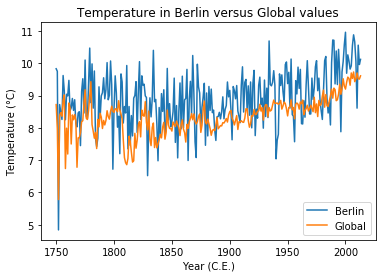
\includegraphics[width=\columnwidth]{AverageTemperaturePlot.png}
		% Create a subtitle for the figure.
		\caption{Simulation results on the AWGN channel. Average throughput $k/n$ vs $E_s/N_0$.}
		% Define the label of the figure. It's good to use 'fig:title', so you know that the label belongs to a figure.
		\label{fig1}
		\end{center}
	\end{figure}
    
    When the data was transformed to fit a 7 year moving average, as can be seen by figure \ref{fig2}, trends become more obvious. This is because taking an average of sections of the data mean that either more varience in a single point is required in order to raise the 7 year average temperature, these conditions can also be satisfied if the temperature raises uniformly over time. The same trend of Berlin having a higher temperature and the presence of large fluctuations in temperatures during the late 1700s is still evident. However, the exponential rise of temperature over time becomes much easier to spot. This is because the temperature is steadily rising instead of having outliers as was often the case before the industrial revolution. This suggests that the forces which are driving the upward in temperatures are compounding themselves. A possible reason for the increase in global temperatures is the increased concentration of carbon dioxide in the atmosphere due to anthropomorphic emissions, but this cannot be concluded from this data alone and more research is required to find a causal link between carbon dioxide concentration and global temperature levels.

	\begin{figure}[!hbt]
		\begin{center}
		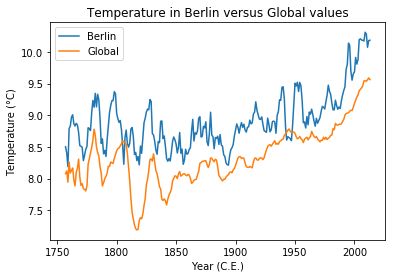
\includegraphics[width=\columnwidth]{7DayMovingAverageTemperaturePlot.png}
		\caption{Seven year moving average of the temperature in Berlin (shown in blue) against the corresponding Global values.}
		\label{fig2}
		\end{center}
	\end{figure}

\newpage

\section{Conclusion}
	In conclusion, there is evidence to suggest that the temperature of the globe has been rising over the past century with the global average rising by roughly 1.5°C. More research is required in order to determine where this change in temperature comes from and what should be done about it if at all and what this could mean for the world.

% Your document ends here!
\end{document}